\documentclass[11pt]{beamer}
\usetheme{Rochester}
\usecolortheme{seagull}
\usepackage[utf8]{inputenc}
\usepackage[german]{babel}
\usepackage[T1]{fontenc}
\usepackage{amsmath}
\usepackage{amsfonts}
\usepackage{amssymb}
\usepackage{textpos}
\usepackage{subcaption}
\usepackage{wrapfig}

% add logo to the sections
\addtobeamertemplate{frametitle}{}{%
\begin{textblock*}{100mm}(.6\textwidth,-1.2cm)

\includegraphics[width=0.5\linewidth]{./logo_inf_fak.png}
\end{textblock*}}


\setbeamertemplate{footline}[frame number]

\author{Größler, Hofmann, Solovjova, Sopauschke, Sturm, Zettwitz}
\title{A Visualization Technique for \\  Hierarchical Edge Bundles}
\date{14.Januar 2016} 
%\setbeamercovered{transparent}  
%\subject{}


\begin{document}

\begin{frame}
\titlepage
\end{frame}

\begin{frame}
\frametitle{Inhalt} 
\tableofcontents
\end{frame}


\section{Ziel des Projekts}
\begin{frame}
\frametitle{Ziel des Projekts}
\begin{itemize} 
\item hierarchische Graphdaten (Baum)
\item Radiales Layout der Graphdaten
\item Bündelung der Graphdaten(Pfade) durch B-Splines
\item Echtzeit/interaktive Visualisierung
\end{itemize}
\end{frame}

\section{Verwendetes Paper}
\begin{frame}
\frametitle{Verwendetes Paper}
\begin{itemize} 
\item Hierarchical Edge Bundles: \\
Visualization of Adjacency Relations in Hierarchical Data
\item Autor: Danny Holten
\item Jahr: 2006
\end{itemize}
\end{frame}

\subsection{Graphenstrukturen}
\begin{frame}
\frametitle{Graphenstrukturen}

\begin{figure}[c]
 
\begin{subfigure}{0.25\linewidth}
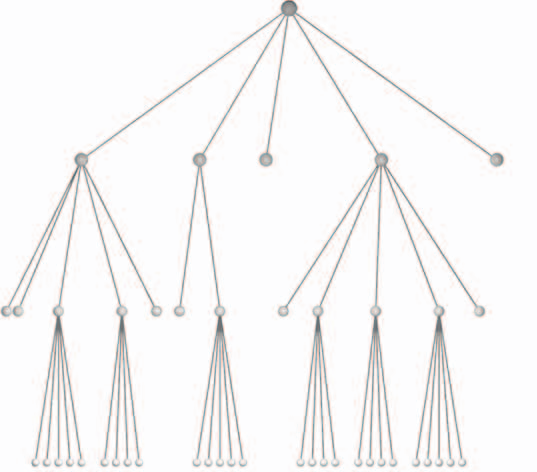
\includegraphics[width=\linewidth, height=2.5cm]{./HierachicalTree.png} 
\caption{Rooted Tree}

\end{subfigure}
 \begin{subfigure}{0.25\linewidth}
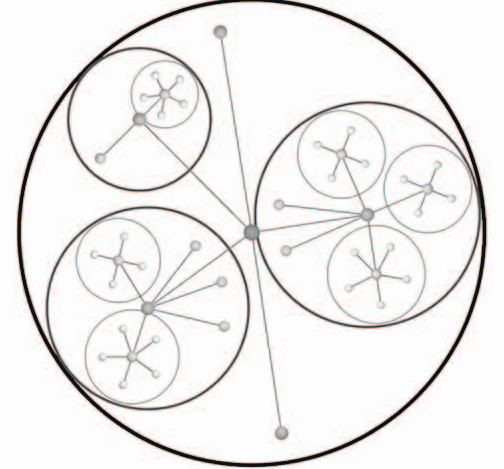
\includegraphics[width=\linewidth, height=2.5cm]{./BalloonTree.png}
\caption{Balloon Tree}

\end{subfigure}
 \begin{subfigure}{0.25\linewidth}
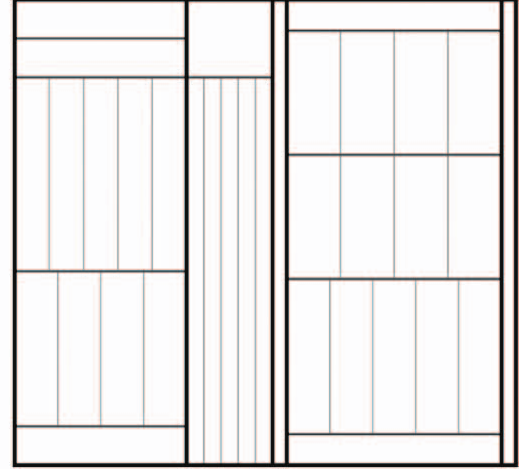
\includegraphics[width=\linewidth, height=2.5cm]{./TreeMap.png}
\caption{Tree Map}
\end{subfigure}
\end{figure}
\end{frame}

\subsection{Radiales Layout}
\begin{frame}
\frametitle{Radiales Layout}
\begin{figure}
\centering
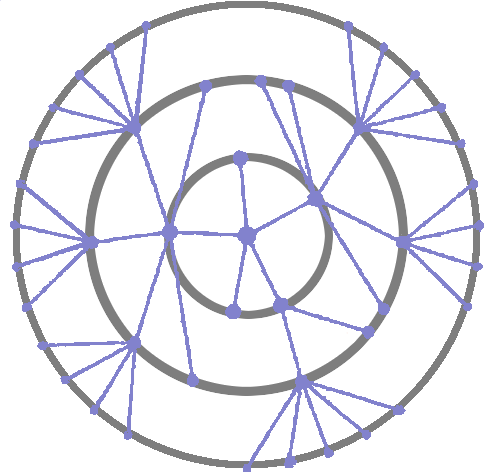
\includegraphics[width=0.6\linewidth]{./RadialTree.png}
\end{figure}
\end{frame}

\subsection{Splines}
\begin{frame}
\frametitle{Splines}\centering
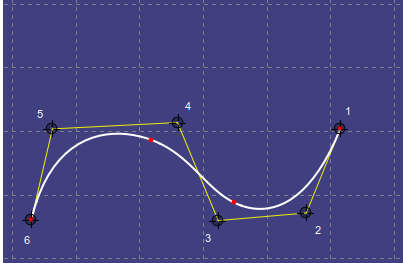
\includegraphics[width=0.6\linewidth]{./CreatedSpline.png}
\begin{itemize}
\item Interpolation bzw. Approximieren zwischen Punkten
\item Beschreibung von Kurven
\item stückweise polynomiale Funktion: 
\end{itemize}
\begin{equation} 
\boxed{\mathbf{x}(t) = \sum_{i = 0}^{n} B_{i}(t) \cdot \mathbf{p}_{i}}
\end{equation}
\end{frame}

\subsection{B-Splines}

\begin{frame}
\frametitle{B-Splines Allgemein}
\begin{itemize}
\item Gegeben sind $n+1$ Kontrollpunkte $\mathbf{d}_0 \text{,}\dots\text{,} \mathbf{d}_n$
\item und ein Knotenvektor $t_0\text{,} t_1\text{,} \dots \text{,} t_{n+k}$
\end{itemize}
\bigskip
\begin{equation}
N_{i,1}(t) = \begin{cases}
                1 & \text{für } t_{i} \leq t < t_{i+1} \\
                0 & \text{sonst}
             \end{cases}
\end{equation}
\begin{equation}
N_{i,k}(t) = \frac{t - t_{i}}{t_{i+k-1} - t_{i}}N_{i,k-1}(t) + \frac{t_{i+k} - t}{t_{i+k} - t_{i+1}}N_{i+1,k-1}(t)
\end{equation}
\bigskip
\begin{equation}
\boxed{\mathbf{x}(t) = \sum_{i = 0}^{n} N_{i,k}(t) \cdot \mathbf{d}_{i}}
\end{equation}

\end{frame}


\begin{frame}
\frametitle{B-Splines Vorteile}
\begin{itemize}
\item Lokaler Einfluss der Kontrollpunkte
\item Niedriger Polynomgrad auch bei vielen Kontrollpunkten
\item Einfügen eines neuen Kontrollpunktes ändert Grad der Kurvensegmente nicht
\end{itemize}
\end{frame}

\begin{frame}
\frametitle{B-Splines Beispiel}
\begin{itemize}
\item Kontrollpunkte $\mathbf{d}_0 \text{ bis } \mathbf{d}_5$
\item $n - 2$ Teilkurven
\item jeweils stückweise kubisch
\end{itemize}
\begin{textblock*}{100mm}(5.5cm,-2cm)
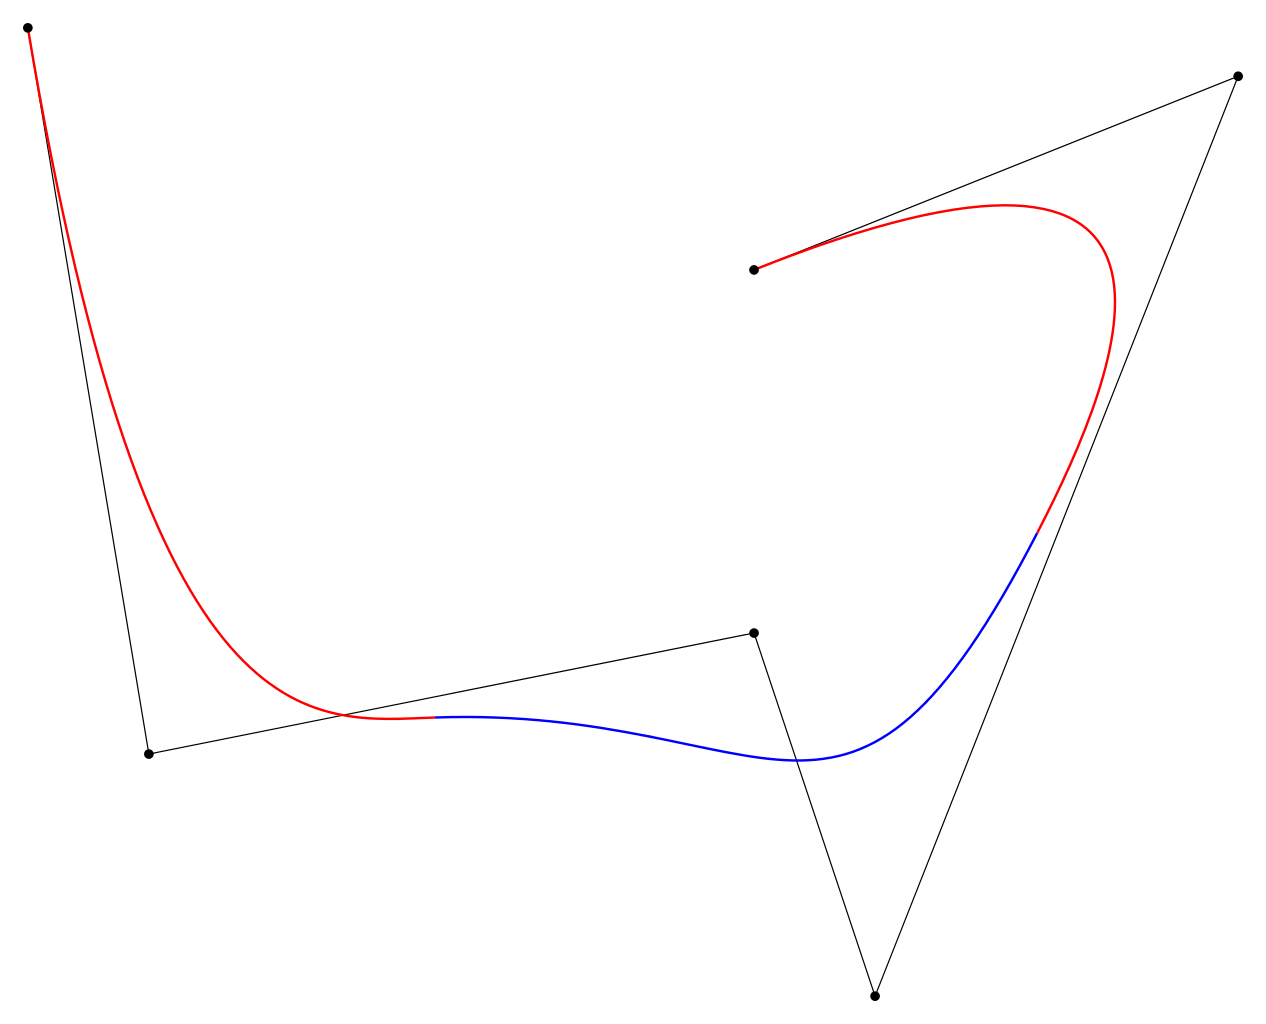
\includegraphics[width=0.6\linewidth]{./B-spline_curve.png}
\end{textblock*}
\end{frame}

\subsection{Der Algorithmus}
\begin{frame}
\frametitle{Skizze des Algorithmus}
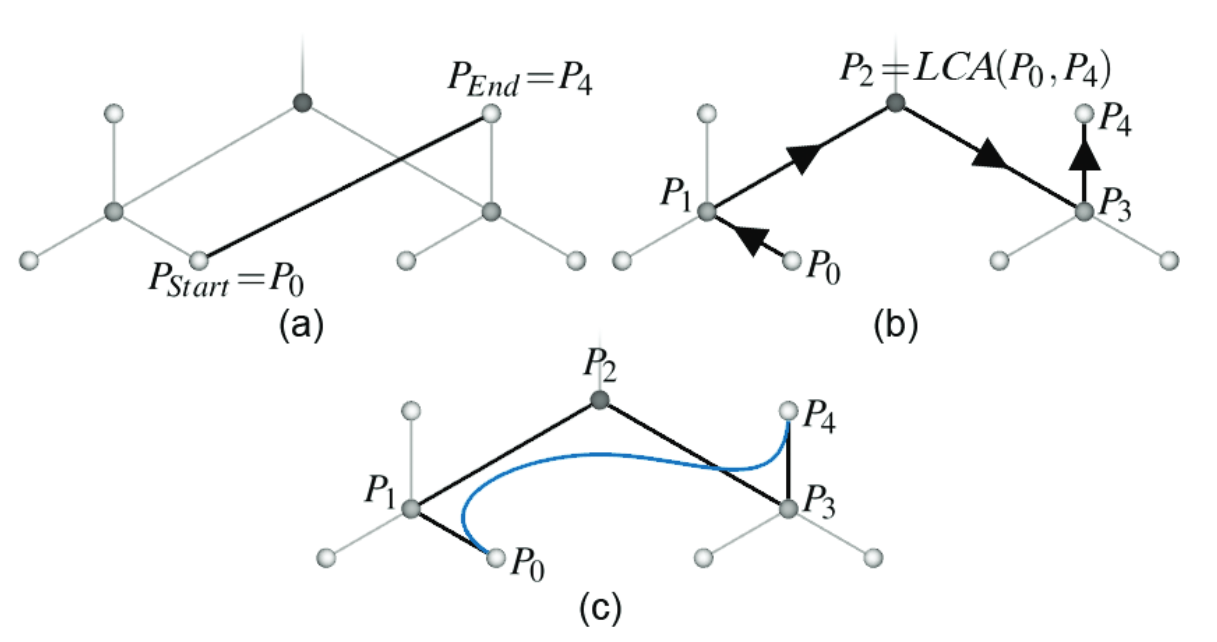
\includegraphics[scale=0.35]{./Algorithm_Scheme.png}
\end{frame}

\begin{frame}
\frametitle{Ergebnis des Algorithmus}
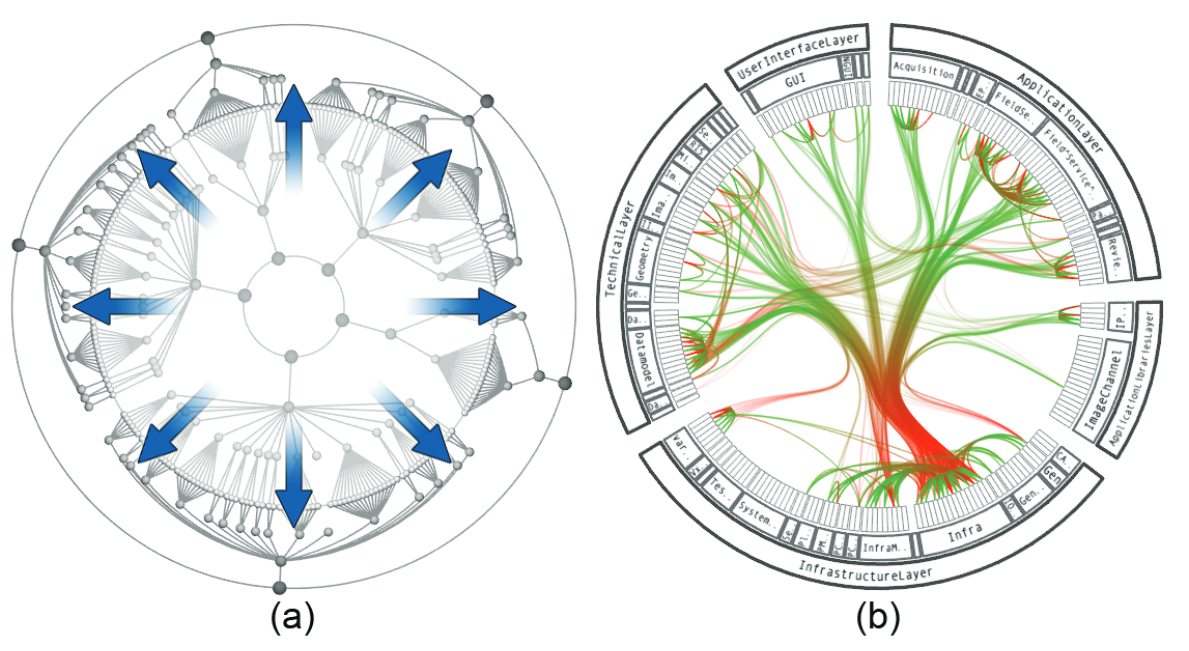
\includegraphics[scale=0.35]{./Algorithm_Result.png}
\end{frame}

\begin{frame}
\frametitle{Anwendung auf anderes Layout}
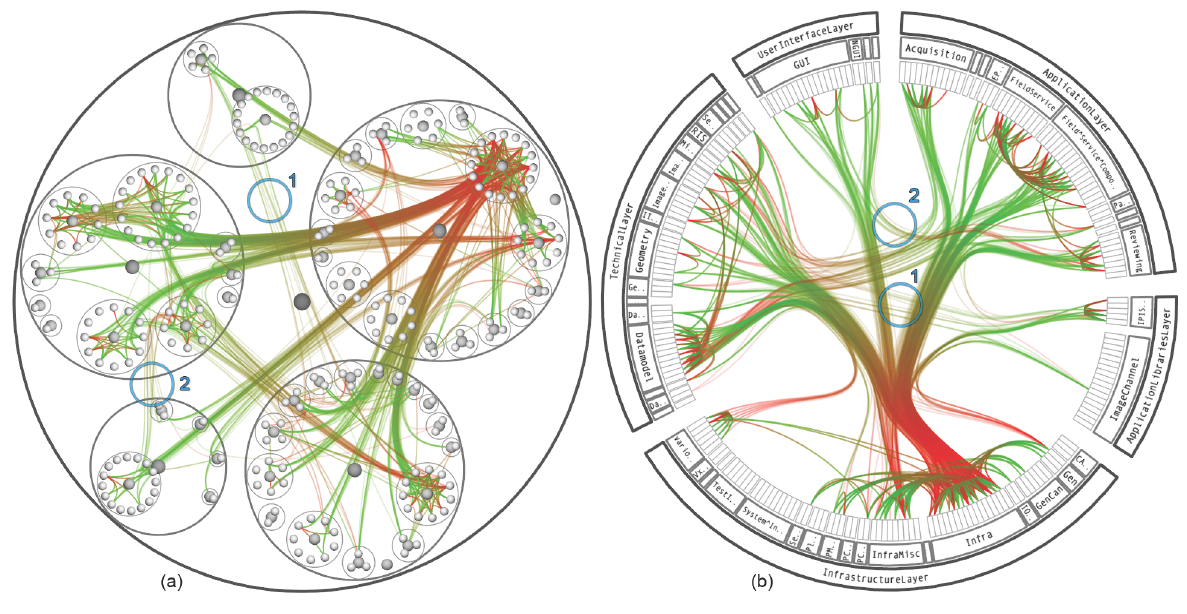
\includegraphics[scale=0.35]{./Algorithm_Result_OtherLayout.png}
\end{frame}

\begin{frame}
\frametitle{Kontrolle der Splines - Beta Faktor}
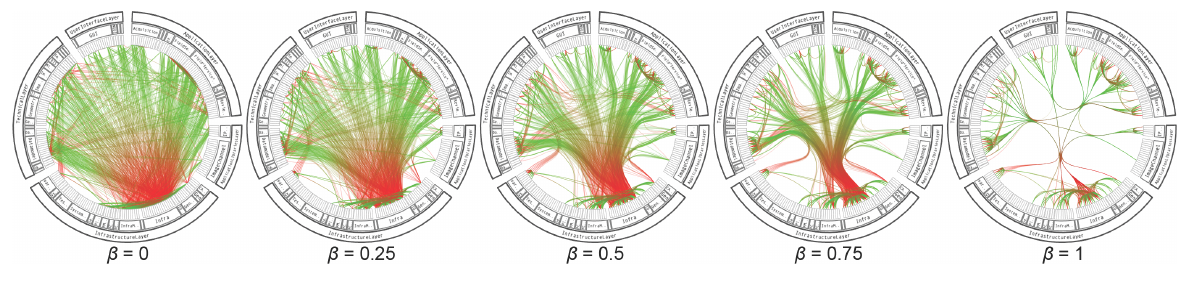
\includegraphics[scale=0.35]{./Algorithm_BetaFactor_Results.png}
\begin{itemize}
\bigskip
\item $\beta$-Faktor steuert Anschmiegen der Splines an Kontrollpolygon
\item hoher $\beta$-Faktor $\rightarrow$ starke Bündelung
\end{itemize}
\end{frame}

\section{Compound Graph}
\begin{frame}[allowframebreaks]
\frametitle{Compound Graph}

Compound Graph Bestandteile:
\begin{itemize} 
\item Wurzel
\item Knoten (Eltern, Kind)                                                                                                                       
\item Level, Link(Ziel), Position(x,y)
\item Anzahl an Kindern auf allen Leveln
\end{itemize}

\begin{figure}
\centering
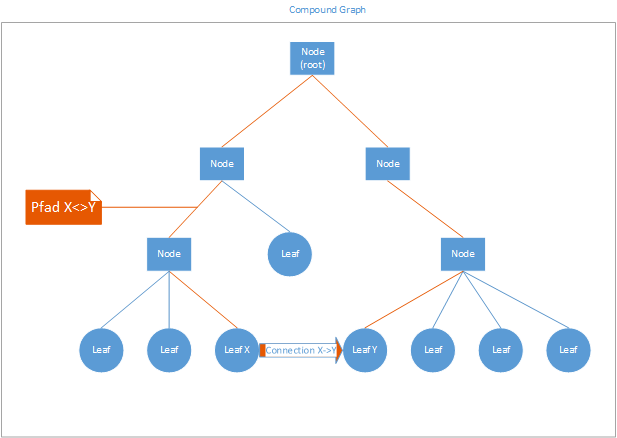
\includegraphics[width=0.79\linewidth]{./Compound_overview}
\caption[Compound_overview]{Übersicht der Baum-/Graphenstruktur}
\label{fig:Compound_overview}
\end{figure}

\framebreak
\begin{itemize} 
\item Pfad nur von Blatt zu Blatt
\item Shortest path: von beiden Endpunkten aufsteigen, \\ bis gemeinsamer Knoten erreicht wurde
\item Speichere jeden besuchten Knoten (später für Splines benötigt)
\item Zufallsgenerierung: \#Level, \#Knoten, \#avg. Kinder, \#Links
\end{itemize}


\begin{figure}
\centering
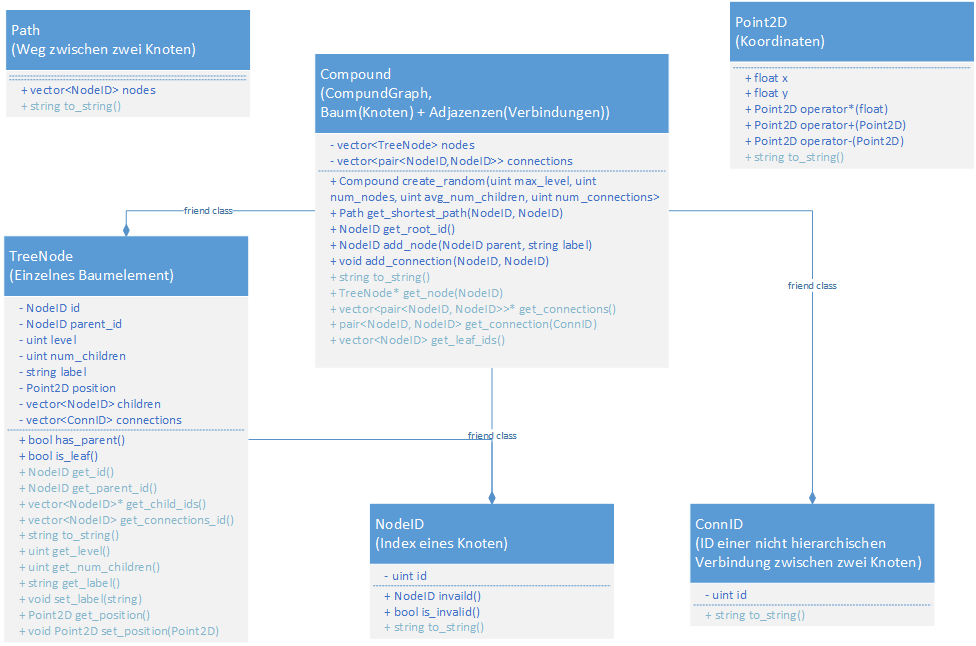
\includegraphics[width=0.85\linewidth]{./UML_tree}
\caption[UML Klassen]{UML Klassendiagramm}
\label{fig:UML_tree}
\end{figure}

\end{frame}


\section{Radiales Layout}
\begin{frame}[allowframebreaks]
\frametitle{Radiales Layout}

\begin{center}
Anzahl aller Kinder bestimmt konzentrisch Position auf Ring 
\\ und bildet Sektor (alle weiteren Kinder innerhalb)\\
\end{center}

\begin{align}
\theta = \frac{\theta_{min} + \theta_{max}}{2} * \frac{\pi}{180} 
\end{align}
\begin{align}
x = radius * \sin(\theta) * level
\\
y = radius * \cos(\theta) * level
\end{align} 

\framebreak
rekursiv für alle [0..i..n] Kinder $c$ unter Knoten $k$:
\begin{align}\theta_{tempMin} = \theta_{tempMax}\end{align}
\begin{align}\theta_{tempMax} = \theta_{tempMin} + (\theta_{max}-\theta_{min})\end{align} 
\begin{align}
\theta_{tempMax} = \theta_{tempMax} * \frac{\Sigma(Kinder_{c[i]})+1}{\Sigma(Kinder_k)}
\end{align}

\framebreak
\begin{figure}
\centering
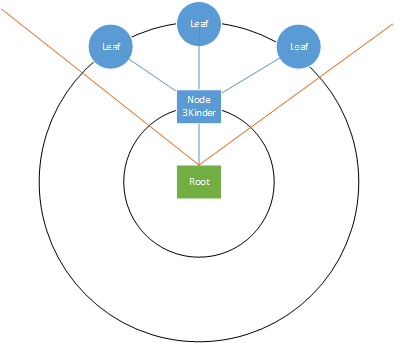
\includegraphics[width=0.6\linewidth]{./radiall}
\caption{Konzept radiales Layout}
\label{fig:radiall}
\end{figure}

\end{frame}

\section{Technisches System}
\begin{frame}
\frametitle{Technisches System}

\begin{itemize}
\item Cross-platform: gestestet unter Windows 8, Ubuntu 14.04, Debian 8
\item Cmake als build-tool für C++ Code
\item OpenGL(GLUT, GLEW) als plattformunabhängige  
\\ Anbindung an Grafikkarte -> schnell(GPU beschleunigt) 
\item Erzeugung des Graphen auf CPU
\item Berechnung der Splines, Rendering auf GPU (Shader)
\item Git als Versionskontrolle und issue tracker
\end{itemize}

\end{frame}

\section{Umsetzung}
\begin{frame}
\frametitle{Umsetzung}

\begin{itemize}
\item zufällige Generierung des Baumes und der Verbindungen
\item Erstellen des radialen Layouts
\item Generieren der Splines
\item Senden aller relevanten Daten an GPU
\item $\beta$-Parameter Manipulation in Shader
\end{itemize}
\end{frame}

\begin{frame}
\frametitle{Shader I}
\begin{itemize}
\item benötigte Daten: 	
	\begin{itemize}
	\item Splinepunkte
	\item $t \in[0,1]$ für Splinepunkt
	\item Länge des Pfades $l_t$
	\item Anfangs-, Endpunkt(für $\beta$)
	\item Farbe von Anfangs-,Endpunkt
	\item $\alpha$-Werte für Blending
	\item $\beta$
	\end{itemize}
\end{itemize}

\end{frame}

\begin{frame}
\frametitle{Shader II}
\begin{itemize}
\item Bestimmung der endgültigen Splineposition durch lineare Interpolation in $\beta$\\
$S`(t)=\beta S(t) + (1-\beta)(P_0 + t(P_{N-1} - P_0))$

\item Bestimmung der Farbe durch lineare Interpolation in $t$ und $l$
$color =(1-t) color_{begin} + t color_{end}$
$opacity = \alpha_{min} \frac{l_t-l_{min}}{l_{max}-l_{min}} + \alpha_{max} (1-\frac{l_t-l_{min}}{l_{max}-l_{min}})$
\end{itemize}
\end{frame}

\section{Demo}
\begin{frame}
\frametitle{Demo}

Es folgt eine kurze Demonstration unserer Ergebnisse

\end{frame}



\section{Grenzen}
\begin{frame}
\frametitle{Grenzen des Programms}

\begin{itemize}
\item Graph erstellen: (Level, Knoten, Kinder, Verbindungen)
\item Grenze unter Linux:
 \begin{itemize} 
 \item bei ca. 2.500.000 Verbindungen (unter 6fps)
 \end{itemize}
\item Grenze unter Windows:
	\begin{itemize}
	\item bei ca. 403.000 Verbindungen (Crash)
	\end {itemize}
\end{itemize}

\end{frame}



\section{Nutzen und Erweiterung}
\begin{frame}
\frametitle{Nutzen und Erweiterung}

\begin{itemize}
\item explorative Datenanalyse
\item visuell ansprechend
\item Erweiterung:
\begin{itemize} 
\item Selektion von Pfaden
\item Zoom- und Filtertechniken
\item lokales Ändern des $\beta$-Parameters 
\item "Hierarchial edge bundles for general graphs" 
\\(Yuntao Jia, Michael Garland and John C. Hart, 2009)
%http://graphics.cs.illinois.edu/sites/default/files/edgebundles.pdf
\end{itemize}
\end{itemize}

\end{frame}


\end{document}
